\documentclass[unknownkeysallowed]{beamer}
\mode<presentation>
{
%  \usetheme{AnnArbor}
%  \usetheme{Dresden}
%  \usetheme{Montpellier}
%  \usetheme{Antibes}
%  \usetheme{Frankfurt}
%  \usetheme{PaloAlto}
%  \usetheme{Bergen}
%  \usetheme{Boadilla}
%  \usetheme{Goettingen}
%  \usetheme{Pittsburgh}	%!!
%  \usetheme{Berkeley}
%  \usetheme{Hannover}
%  \usetheme{Rochester}		%!!!
%  \usetheme{Berlin}
%  \usetheme{Ilmenau}
%  \usetheme{Singapore}
  \usetheme{Boadilla}		%viel platz
%  \usetheme{JuanLesPins}
%  \usetheme{Szeged}		%!
%  \usetheme{boxes}
%  \usetheme{Luebeck}
%  \usetheme{Warsaw}
%  \usetheme{Copenhagen}
%  \usetheme{Madrid}
%  \usetheme{Darmstadt}
%  \usetheme{Malmoe}
%  \usetheme{default}
%  \usetheme{JuanLesPins}

%  \usetheme{Marburg}


%\usefonttheme{professionalfonts}
%	default | professionalfonts | serif |
%	structurebold | structureitalicserif |
%	structuresmallcapsserif
%\useinnertheme{rounded}
%	circles | default | inmargin |
%	rectangles | rounded

%  \setbeamercovered{transparent}
  % oder auch nicht
\usecolortheme{rose}


\definecolor{uaf yellow}{cmyk}{0,0.16,1,0} % official UAF yellow
\definecolor{light yellow}{cmyk}{0.01,0,0.16,0}
\definecolor{uaf blue}{cmyk}{1,0.66,0,0.02} % official UAF blue
\definecolor{light blue}{cmyk}{0.22,0.11,0,0}
\definecolor{arsc blue}{HTML}{005496}
\definecolor{arsc red}{HTML}{a20a42}
\definecolor{arsc green}{HTML}{009a82}
\definecolor{light gray}{HTML}{777777}

  %navigation aus, klaut nur platz
  \setbeamertemplate{navigation symbols}{}
% Reset title background to default
%\setbeamertemplate{title page}[default]
\setbeamercolor{title}{bg=}
\setbeamercolor{frametitle}{bg=uaf blue, fg=white}
\setbeamercolor{institute}{fg=white}
\setbeamercolor{date}{fg=white}
\setbeamercolor{block}{bg=}
%\setbeamercolor{title}{fg=black}

% Reset block background to default
%\setbeamertemplate{blocks}[default]
%\setbeamercolor{block title}{bg=}
%\setbeamercolor{block body}{bg=}

\beamertemplatenavigationsymbolsempty  
\setbeamertemplate{blocks}[rounded][shadows=false]

\useinnertheme{circles}

}
\usepackage[latin1]{inputenc}
\usepackage{latexsym}
\usepackage{amsfonts}
%\usepackage{natbib}
\usepackage{fancyhdr}
\usepackage{graphicx}
%\usepackage{subfigure}
% oder was auch immer
\usepackage{grffile}
\usepackage{pgf}
\usepackage{tikz}

\usepackage{listings}

\usepackage{times}
\usepackage[T1]{fontenc}
%\usepackage{appendixnumber}
% Oder was auch immer. Zu beachten ist, das Font und Encoding passen
% müssen. Falls T1 nicht funktioniert, kann man versuchen, die Zeile
% mit fontenc zu löschen.

\hypersetup{
    bookmarks=true,         % show bookmarks bar?
    unicode=false,          % non-Latin characters in Acrobat's bookmarks
    pdftoolbar=true,        % show Acrobat's toolbar?
    pdfmenubar=true,        % show Acrobat's menu?
    pdffitwindow=false,     % window fit to page when opened
    pdfstartview={FitH},    % fits the width of the page to the window
    pdftitle={My title},    % title
    pdfauthor={Author},     % author
    pdfsubject={Subject},   % subject of the document
    pdfcreator={Creator},   % creator of the document
    pdfproducer={Producer}, % producer of the document
    pdfkeywords={keyword1} {key2} {key3}, % list of keywords
    pdfnewwindow=true,      % links in new window
    colorlinks=false,       % false: boxed links; true: colored links
    linkcolor=red,          % color of internal links
    citecolor=green,        % color of links to bibliography
    filecolor=magenta,      % color of file links
    urlcolor=cyan           % color of external links
}

\title[PAG]% (optional, nur bei langen Titeln nötig)
{GEOS 436 / 636\\
Programming and Automation for Geoscientists\\[20pt]
-- Week 11: Debugging \& Examples --
}

\author[Grapenthin]% (optional, nur bei vielen Autoren)
{Ronni Grapenthin\\
rgrapenthin@alaska.edu\\
Elvey 413B\\
x7682}
% - Namen müssen in derselben Reihenfolge wie im Papier erscheinen.
% - Der \inst{?} Befehl sollte nur verwendet werden, wenn die Autoren
%   unterschiedlichen Instituten angehören.

\institute[UAF] % (optional, aber oft nötig)
{}
% - Der \inst{?} Befehl sollte nur verwendet werden, wenn die Autoren
%   unterschiedlichen Instituten angehören.
% - Keep it simple, niemand interessiert sich für die genau Adresse.

% - Namen müssen in derselben Reihenfolge wie im Papier erscheinen.
% - Der \inst{?} Befehl sollte nur verwendet werden, wenn die Autoren
%   unterschiedlichen Instituten angehören.

% - Der \inst{?} Befehl sollte nur verwendet werden, wenn die Autoren
%   unterschiedlichen Instituten angehören.
% - Keep it simple, niemand interessiert sich für die genau Adresse.

\date[]{}

% - Volle oder abgekürzter Name sind möglich.
% - Dieser Eintrag ist nicht für das Publikum gedacht (das weiß
%   nämlich, bei welcher Konferenz es ist), sondern für Leute, die diese
%   Folien später lesen.

%\AtBeginSection[]
%{
%  \begin{frame}<beamer>
%    \frametitle{Outline}
%    \tableofcontents[currentsection,currentsubsection]
%  \end{frame}
%}

% Falls Aufzählungen immer schrittweise gezeigt werden sollen, kann
% folgendes Kommando benutzt werden:

%\beamerdefaultoverlayspecification{<+->}

%%switch on to have only frame numbers
\setbeamertemplate{footline}[frame number]

\defbeamertemplate*{title page}{customized}[1][]
{
		\begin{tikzpicture}
			\node[text width=\textwidth,
				fill=gray!70, 
				fill opacity=0.75,
				text opacity=1,
				rounded corners = 10pt,
				inner sep=2pt]{
				\begin{center}	
			  \usebeamerfont{title}{\bf \usebeamercolor[fg]{title} \inserttitle}
			  \par
			  \usebeamerfont{subtitle}\insertsubtitle\par
			  \bigskip
			  \usebeamerfont{author}\insertauthor\par
			  \bigskip
			  \usebeamerfont{institute}\insertinstitute\par
			  \bigskip
			  \usebeamerfont{date}\insertdate\par
			  \end{center}
			  };
	\end{tikzpicture}		  
%	\vspace{0.4cm}\usebeamercolor[fg]{titlegraphic}\inserttitlegraphic 
%	\begin{flushright}
%	\vspace{-1.25cm}\includegraphics[width=2cm]{../moore_logo_transp.png}\vspace{5cm}
%	\end{flushright}
}

\begin{document}

\lstset{numbers=left, numberstyle=\tiny, stepnumber=2, basicstyle=\ttfamily, numbersep=5pt, xleftmargin=10pt}

\setbeamertemplate{background}{\includegraphics[width=\paperwidth]{/home/roon/Pictures/rooftop_initial.jpg}}

	\begin{frame}
	\begin{center}
		\titlepage
	\end{center}
	\end{frame}

\setbeamertemplate{background}{}

\begin{frame}
\frametitle{}
%	\vspace{2cm}
	\begin{center}
	The code doesn't work!\\[10pt]
	How do we fix it?
	\end{center}
\end{frame}

\begin{frame}
	\frametitle{Review: Software Development Cycle}
	\begin{enumerate}
		\item Design
		\item Coding
		\item Test
		\item {\bf Debugging}
		\item go back to 1, 2, 3, \dots
	\end{enumerate}
	\begin{center}	
	This cycle is common to all programming strategies, independent of how involved each stage is. 
	\end{center}	
\end{frame}

\begin{frame}
	\frametitle{What is ``Debugging''?}
	\begin{block}{}
	Debugging is the {\bf art} of finding and fixing mistakes in computer
	programs. To be successful you need insight, creativity, logic, and
	determination.
	\end{block}

	\begin{block}{}
	\emph{Debugging is twice as hard as writing the code in the first
	place. Therefore, if you write the code as cleverly as possible,
	you are, by definition, not smart enough to debug it.
	}
	\begin{flushleft}
	\tiny{Brian Kernighan}
	\end{flushleft}	
	\end{block}

\end{frame}

\begin{frame}
	\frametitle{Simple Truths about Bugs and Debugging \dots}
	\begin{itemize}
		\item Bugs are static -- they won't run away.
		\item Often, the problem is simple.
		\item You created the code, so you made the bug! It's nobody else's fault - get to it!
		\item Debugging is a great way to learn being self-critical. Good luck!
		\item Be critical -- did you mean `<', `<=', `>', `>='?
		\item Don't panic -- be systematic!
		\item Sleep, go for a walk, come back later.
	\end{itemize}
\end{frame}

\begin{frame}
	\frametitle{Debugging Styles / Helpful Tools}

	\begin{itemize}
		\item {\bf echoing:} place print statements at useful points in a program (function entry, exit)
		\item {\bf unit testing:} write calls to particular function, throw artificial values at it, automate this to test units with every change of the code
		\item {\bf exception handling:} in high level languages: sources of mistakes easier to spot
		\item {\bf online debuggers:} for our purposes usually not necessary, useful if you want to step through your code, or for memory problems
		\item {\bf version control:} have a tool keep track of changes you make; roll back or comparisons to bug-free code is simple (not covered here)
	\end{itemize}
\end{frame}
	

\begin{frame}
	\frametitle{Debugging Styles: Echoing vs. Online Debuggers}
	\begin{block}{}
	\emph{\dots we find stepping through a program less productive than
		thinking harder and {\bf adding output statements and
		self-checking code at critical places}. Clicking over
		statements takes longer than scanning the output of
		judiciously-placed displays. It takes less time to decide where
		to put print statements than to single-step to the critical
		section of code, even assuming we know where that is. More
		important, {\bf debugging statements stay with the program;
		debugging sessions are transient}.}
	\begin{flushleft}
	\tiny{\emph{From: Brian Kernighan, Rob Pike ``The Practice of Programming''}}
	\end{flushleft}	
	\end{block}
\end{frame}

\begin{frame}
	\frametitle{Debugging Styles: Echoing}
	\begin{itemize}
	\item at the simplest: supplement your code with {\tt print()} or {\tt echo} statements where necessary
	\item more sophisticated: 
		\begin{itemize}
			\item write a function that displays text only if a global DEBUG flag is set.
			\item call this function whenever necessary: entry or exit of function, display variable values before / after critical operations, to follow the program flow, \dots
			\item turn DEBUG off when everything works
		\end{itemize}
	\end{itemize}
\end{frame}

\begin{frame}
	\frametitle{Debugging Styles: Unit Testing}
	\begin{itemize}
		\item at the simplest: write a script that calls your functions with artificial values and compares results to expected outcome
		\item execute whenever code changes are made
		\item helps to detect errors due to changes in functions immediately
		\item possible for any language (fancy frameworks exist for some languages)
	\end{itemize}
\end{frame}


\begin{frame}
\frametitle{Debugging Styles: Unit Testing}
	\begin{center}
		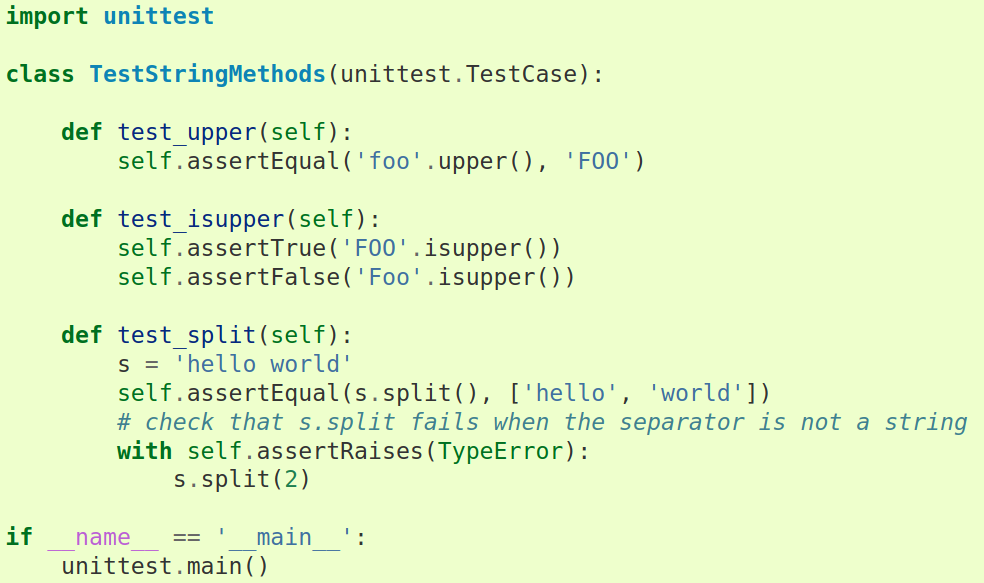
\includegraphics[width=.8\textwidth]{../figures/python_unittest.png}	
	\end{center}
	\begin{flushleft}
	\tiny{\emph{\url{https://docs.python.org/}}}
	\end{flushleft}	
\end{frame}

\begin{frame}
\frametitle{Debugging Styles: Exception Handling}
	\begin{center}
	The motto: Keep the program running in cases where things go wrong (in recoverable ways).
	\end{center}
	\begin{center}
		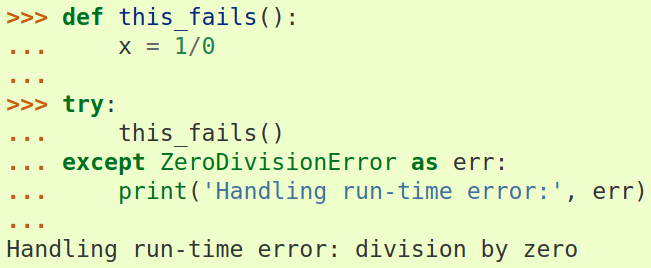
\includegraphics[width=.8\textwidth]{../figures/python_exception_handling.png}	
	\end{center}
	\begin{flushleft}
	\tiny{\emph{\url{https://docs.python.org/}}}
	\end{flushleft}	
\end{frame}


\end{document}
